\documentclass[12pt,fleqn]{article}\usepackage{../../common}
\begin{document}
Ders 2

Çoğunlukla özvektör kavramına atıf yapıldığında söylenmek istenen ($C$
kompleks sayıların kümesi olsun),

$$ Av = \lambda v, \qquad \lambda \in C $$

ifadesidir, yani ``sağ özvektör'', yani bir matrisi {\em sağdan} çarpınca
boyu büyüyen ya da küçülen vektör. Sol özvektörler de mümkün, bu durumda, 

$$ v^TA = \lambda v^T, \qquad \lambda \in C $$

$A$'nin spektrumu $\sigma(A)$ o matrisin tüm özvektörlerinin
kümesidir. Numpy ile

\begin{minted}[fontsize=\footnotesize]{python}
import numpy.linalg as lin
A = [[3,4,3],[5,5,6],[5,5,5]]
A = np.array(A)
[V,D] = lin.eig(A)
print 'ozvektorler'
print D
print 'ozdegerler'
print V
\end{minted}

\begin{verbatim}
ozvektorler
[[-0.41963784+0.j          0.72738656+0.j          0.72738656-0.j        ]
 [-0.66394149+0.j         -0.42567121+0.33744486j -0.42567121-0.33744486j]
 [-0.61893924+0.j         -0.25117492-0.33579002j -0.25117492+0.33579002j]]
ozdegerler
[ 13.75351937+0.j          -0.37675969+0.47073926j  -0.37675969-0.47073926j]
\end{verbatim}

Eğer $B = PAP^{-1}$, ki $P$ eşsiz olmayacak şekilde, o zaman $\sigma(B) =
\sigma(A)$. İspatsız veriyoruz. Yani $P$ ve onun tersi ile bir matrisi iki
taraftan çarpmak, o matrisin spektrumunu değiştirmiyor.

Eğer $\lambda \in C$ bir özdeğer ise, onun eşleniği (conjugate)
$\bar{\lambda}$ da bir özdeğerdir. Bu sebeple reel matris $A$ için
$\sigma{A} = \overline{\sigma{A}}$. 

Bir reel matrisin tüm özdeğerlerinin reel olduğu ``güzel'' bir durum
vardır; bu durum matrisin simetrik olduğu durumdur, yani $S^T = S$. Bu
güzel durum aslında pratikte pek çok kez karşımıza çıkar; mesela kovaryans
matrisleri olarak.

Simetrik matrisin özgün özdeğerlerine tekabül eden özvektörleri birbirine
dikgendir. İspat, $v_i^T S v_j $ formülüne bakalım, ki $v_i,v_j$
özvektörler, $S$ simetrik matris.

Özdeğer eşitliğinden $S v_j = \lambda_j v_j$ kullanırsam,

$$ v_i^T S v_j  = \lambda_j v_i^T v_j $$

Eğer  $v_i^TS = \lambda_i v_i^T$ kullanırsam,

$$ v_i^T S v_j  = \lambda_i v_i^T v_j $$

elde ederim. İkisini bir araya koyalım,

$$ \lambda_j v_i^T v_j =  \lambda_i v_i^T v_j $$

$$ (\lambda_j-\lambda_i) v_i^T v_j = 0$$

Bu eşitliğin doğru olması sadece iki durumda olabilir; ya
$\lambda_i,\lambda_j$ birbiriyle aynıdır, ya da birbirinden farklıdır ama
o zaman  $v_i,v_j$ birbirine dikgen olmalıdır. 

[norm atlandı]

Eksi Bakışımlı Matrisler (Skew-symmetric Matrices)

Eğer $A^T = -A$ ise bu matrislere eksi bakışımlı deniyor [5]. Mesela

$$ 
\left[\begin{array}{rr}
0 & 2 \\ -2 & 0
\end{array}\right]
 $$

Bu matrisin devriği ve negatifi aynıdır. Eksi bakışımlı matrislerin
köşegeni sıfır olmalıdır. Bu tür matrislerin ilginç bazı özellikleri var,
mesela, hatırlarsak simetrik matrislerin pür reel spektrumu vardı. Eksi
bakışımlı matrislerin spektrumu pür sanaldır (imaginary).

[köşegenleştirme atlandı]

Çapraz Çarpım (cross-product) 

Noktasal çarpım bize bir skalar verir. İki vektör arasındaki çapraz çarpım
bize başka bir vektör verir; $u,v \in \mathbb{R}^3$ olmak üzere çapraz çarpım,

$$ 
u \times v = 
\left[\begin{array}{r}
u_2v_3 - u_3v_2 \\
u_3v_1 - u_1v_3 \\
u_1v_2 - u_2v_1 
\end{array}\right]
$$

Yani $\mathbb{R}^3$'teki iki vektör $u,v$'nin çapraz çarpımı alınabilir, ve
$\mathbb{R}^3$'te yeni bir vektör elde ederiz. Bu yeni vektör $u,v$'ye
dikgendir. Sağ el kuralı (alttaki resimde $u,v$ yerine $a,b$ kullanılmış)

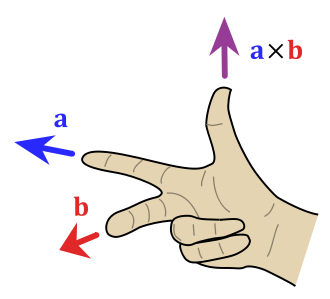
\includegraphics[height=3cm]{righthand.png}

Ayrıca çapraz çarpım simetriktir, $u \times v = - u \times v$. 

Eksi Bakışımlı Matris (Skew-Symmetric Matrix)

Bilgisayar Görüşü (Computer Vision) alanında oldukça yaygın bir matris olan
eksi bakışımlı bir matris alttadır, ve onu herhangi bir vektörden oluşturan
şapka operatörüyle gösterelim, yani $u$ için $\hat{u}$ olsun,

$$ 
\hat{u} = \left[\begin{array}{rrr}
0 & -u_3 & u_2 \\
u_3 & 0 & -u_1 \\
-u_2 & u_1 & 0
\end{array}\right] \in \mathbb{R}^{3 \times 3}
 $$

Bu tür matrislerin kertesinin çift sayı olması şarttır.

$\hat{u}$'nun ilginç bir özelliği var, herhangi bir vektör $v$ ile

$$ \hat{u}v = u \times v $$

ki $\times$ bir çapraz çarpım. Yani, öncelikle, her vektörün bir eksi
bakışımlı matris karşılığı var, ve üstteki operatör ile bu geçişi
yapabiliriz, ayrıca ne zaman bir çapraz çarpım görsek, onu eksi bakışımlı
matris çevirimi üzerinen bir normal matris çarpımı olarak temsil
edebiliriz. Bu faydalı çünkü çapraz çarpımla uğraşmak biraz külfetli
olabiliyor. 

3 boyut bağlamında $\hat{u}$'nun kertesi tabii ki 2'dir; çünkü eksi
bakışımlı matrislerinin kertesinin çift olması şart ise, ve 3 boyutlu
durumda bu kerte en fazla 3 olabilir, ama 3 olamaz çünkü 3 çift sayı değil,
o zaman 2 olur.

\inputminted[fontsize=\footnotesize]{python}{skew.py}

\begin{minted}[fontsize=\footnotesize]{python}
A = np.array([[1,2,3]]).T
print skew(A)
\end{minted}

\begin{verbatim}
[[ 0 -3  2]
 [ 3  0 -1]
 [-2  1  0]]
\end{verbatim}

$A^3$

Diyelim ki $A$ bir $3 \times 3$ eksi bakışımlı matris, ve $a =
(a_1,a_2,a_3)$ vektörü üzerinden oluşturulmuş. $A^3$ nedir? 

$$A \cdot x = u \times x$$

olduğunu biliyoruz. O zaman 

$$A^3 x = a \times ( a \times ( a \times x))$$

demektir. Eşitliğin sağ tarafına bakarsak, eğer $a=e$, ki $e$ bir birim vektörü
olsun, yani $||e||=1$, o zaman norm'ların ilişkisi şu şekilde olurdu,

$$||e\times(e\times (e\times x)))\|=||e\times (e\times x))|| =||e\times x||$$

Neden? 

$$ ||e \times x|| = ||e||||x|| \sin \theta = ||x|| \sin \theta$$

O zaman,

$$||e\times (e\times x))|| = ||e|||| e \times x|| \sin 90 = ||e \times x||$$

Böyle gider. Yani norm eşitlikleri doğru. 

Eğer $a = ||a||e$ kabul edersek,

$$||a\times(a\times (a\times x)))|| = ||a||^3 ||e\times(e\times (e\times x)))||$$

$$ =\|a\|^3\|e\times x\| $$

$$ =\|a\|^2\|a\times x\| $$

$$ =(a^Ta)\|a\times x\| $$

Yani $A^3x = \pm (a^Ta) Ax$; eksi mi artı mı? Eksi işareti olduğunu sağ el
kuralıyla görebiliriz. Demek ki $A^3 = -(a^Ta) \cdot A$. 

Simetrik matrisler için 

$$ A = UDU^T $$ 

olduğunu biliyoruz. Eksi bakışımlı matrisler için 

$$ S = UBU^T $$

olur ki $B$ bir blok köşegen matristir, $U$ dikgen. $S$'in özdeğerleri pür
sanaldır. Blok köşegen matris $diag(a_1Z,a_2Z,...,z_mZ,0,..0)$, ve $Z =
\left[\begin{array}{cc} 0 & 1 \\ -1 & 0 \end{array}\right]$. 
Köşegende blok olması garip gelebilir, fakat tek sayılar yerine çapraz
yönde birkaç sayının ``üst üste'' olduğu bir durum bu. Basit matris
çarpımı ile kolay bir şekilde kontrol edilebilir ki

$Z^2 = -I, \qquad Z^3 = -Z, \qquad Z^4 = I$

Matris Üstelleri (Matrix Exponentials) [1, sf. 482]

$t \in \mathbb{R}$ ve bir kare matris $n \times n$ matrisi $A$ için, matris üsteli,

$$ U(t) = e^{tA} = \exp(tA) $$

alttaki problem için özgün bir $n \times n$ çözümüdür;

$$ \frac{dU}{dt} = AU, \qquad U(0) = I $$

Dikkat: matris üsteli $\exp$ fonksiyonun teker teker matris öğeleri
üzerinde işletilmiş hali değildir.

Matris üstelleri bir seri olarak ta gösterilebilir, 

$$ e^{tA} = \sum_{n=0}^{\infty} \frac{t^n}{n!} A^n = 
I + tA + \frac{t^2}{2}A^2 + \frac{t^3}{6}A^3 + ...
$$

Bu seri yakınsayan (converging) bir seridir. 

Örnek

$$ A = \left[\begin{array}{rrr}
0 & 1 \\ 0 & 0
\end{array}\right] $$

için 

$$ e^{tA} = \left[\begin{array}{rrr}
1 & t \\ 0 & 1
\end{array}\right] $$

Örnek

$$ A = \left[\begin{array}{rrr}
1 & 0 \\ 0 & 1
\end{array}\right] $$

için 

$$ e^{tA} = \left[\begin{array}{rrr}
e^t & 0 \\ 0 & e^t
\end{array}\right] $$

Teori 

Eğer $A$ bir eksi bakışımlı matris ise, $Q(t) = e^{tA}$ muntazam 
(proper) bir dikgen matristir. 

İspat 

Dikgenlik tersi ile devriğin aynı olması demektir, o zaman üstteki
eşitlikte sol tarafın tersi, sağ tarafın devriği aynı olmalı, yani
$Q(t)^{-1}$ ile $e^{tA^T}$.

$$ Q(t)^{-1} = e^{-tA} = e^{tA^T} = (e^{tA})^T = Q(t)^T $$

Hakikaten de öyle. 

Not: Bir diğer ispata göre {\em tüm} dikgen matrisler bir eksi bakışımlı
matrisin $e$'nin üsteli alınarak oluşturulabilir. Buradaki nüansa dikkat,
tüm eksi bakışımlı matrislerin üsteli dikgendir demek ile {\em tüm} dikgen
matrisler eksi bakışımlı matrislerin üsteli alınmış halidir demek farklı.

Üstteki kavramları kullanarak dönüş (rotation) yapmayı sağlayan Rodriguez
formülü [6]'da bulunabilir.

SVD 

Bu işlemin özdeğer / özvektör hesabının karesel olmayan matrisler
durumundaki genelleştirilmiş hali olduğu düşünülebilir. Pek çok lineer
cebir işlemi, mesela tersini alma, kerte hesabı, vs. SVD bağlamında
incelenebilir. Genelleştirme dedik, eğer $A$ karesel değilse özvektörleri
hesaplayamayız, ama $A^TA$ kareseldir, ve bu matrisin özvektörleri $A$'nin
SVD'si ile yakından alakalıdır.

[İspat atlandı]

Geometrik olarak $A = U \Sigma V^T$ ile gösterilen SVD'nin bir $x \in
\mathbb{R}^n$'yi $A$ uzerinden transform ettiğimiz durumda, $y = Ax$
diyelim, $y$'nin $U$'da bazındaki kordinatlarının $V$ bazındaki
kordinatları ile bir ilişki ortaya çıkarttığını söyleyebiliriz; bu ilişki
$\Sigma$'nin öğeleri üzerinden bir ölçeklemeden ibarettir. Yani

$$ y = Ax = U\Sigma V^Tx 
\quad \Leftrightarrow \quad
U^Ty = \Sigma V^T x
$$

[birim küre ellipsoid eşlemesi atlandı]

Genelleştirilmiş Ters (Generalized -Moore Penrose- Inverse)

Lineer sistem çözerken $Ax = b$ için eğer $A$'nin tersi alınabiliyorsa,
çözüm kolay, $x^\ast = A^{-1}b$. Fakat $A$'nin tersi alınamıyorsa, ki bu $A$
karesel olmadığında otomatik olarak doğru olacaktır, ne yapacağız?
Genelleştirilmiş tersi alma, ya da sözde ters (pseudoinverse) işlemi burada
ise yarar. Sözde ters için, her $A$ için bir SVD olduğuna göre, $A = U
\Sigma V^T$, ve $\Sigma$'nın sıfır olmayan eşsiz değerlerinin tersi alınır (yani 
öğe $\sigma_i$, $1/\sigma_i$ olur), sıfır değerlerine dokunulmaz, bu sonuçlar yeni 
bir $\Sigma^{\dagger}$'in köşegenine dizilir, ``sözde ters'' bu matris olur,

$$ \Sigma^{\dagger} = \left[\begin{array}{cc}
\Sigma_1^{-1} & 0 \\ 0 & 0 
\end{array}\right]$$

Ve bu ters işlemi tüm $A$'nin tersini almak için kullanılır, ki bu sözde
tersi de boyutu $n \times m$ olan bir $A^{\dagger}$ ile gösteriyoruz
(İngilizce ``$A$-dagger'' olarak telafuz ediliyor, biz ``$A$-kama''
diyelim), 

$$ 
A^{\dagger} = V \Sigma^{\dagger} U^T  
\mlabel{1}
$$

Bu noktaya nasıl geldiğimize dikkat, eğer SVD sonucunun pür tersini
alabilseydik, 

$$ A^{-1} = V^{-T}\Sigma^{-1}U^{-1} $$

Dikgen matrisler için $Q^{-1}=Q^T$ olduğu için 

$$ = V\Sigma^{-1}U^{T} $$

$\Sigma^{-1}$ olmadığı için yerine $\Sigma^{\dagger}$ kullanıyoruz ve (1)'e erişiyoruz.  

Bazı özellikler,

$$ A A^{\dagger} A = A $$

ya da

$$ A^{\dagger} A  A^{\dagger} =  A^{\dagger} $$

Peki sözde tersi alma işlemini denklem sistemi çözmekte nasıl kullanırız? 

Lineer sistem çözümü bağlamında durumunda 3 türlü sonuç olabileceğini
görmüştük. Eğer sonsuz tane çözüm varsa, bu büyük bir ihtimalle problemin
tam kısıtlanmamış (constrained) olması ile alakalıdır. Tabii hiçbir çözüm
olmayabilir, ve size para veren kişi sizden hala çözüm beklemektedir (!),
bu durumda $Ax=b$'yi çözmek yerine ona en yakın olabilecek şeyi
çözebiliriz, yani $|Ax - b|^2$'yi minimize etmeyi seçebiliriz, $Ax$'i
$b$'yi mümkün olduğu kadar yaklaştırırız. Burada sözde ters ise yarar,
çünkü $x^\ast = A^{\dagger}b$ ile hesaplanan çözüm aynı zamanda $|Ax - b|^2$'yi
minimize eder! Bu çözüm En Az Kareler (Least Squares) çözümü olarak ta
bilinir, tabii burada sistem aşırı belirtilmiş (overdetermined) değil,
eksik belirtilmiş (underdetermined) durumda. Not: Ayrıca sözde ters ile
bulunan $x^\ast$'in mümkün tüm çözümler arasında ``norm'ü en az olan $x^\ast$'i
bulduğu da'' söylenir.

Eğer çözüm özgün ise, sözde ters yine işler, özgün çözümü bulur. Yani her
halükarda sözde ters tüm problemlerimizi çözer.

Lineer cebir'i böylece gözden geçirmiş olduk. Artık dersimizin ana
konularına başlayabiliriz. 

Hareketli bir Sahneyi Temsil Etmek

Burada sahne dış dünya, yani kamera ile hareket ederken gördüğümüz şeyler. 

Hareket ederken kamera pek çok resim alabilir, tabii bu dersimiz uzun
zamandır yapılan araştırmalara dayanıyor, ve bu araştırmalar çoğunlukla iki
resim durumuna odaklandılar; fakat günümüzde bir kamera saniyede mesela 30
tane resim çekebilir, bu durum için gerekli matematiği de göreceğiz. Önce
iki resimle başlayacağız, ve bu matematiğin daha genel, çok resimli haline
de kendimizi hazırlayacağız. 

3D'de Yeniden Oluşturmak (3D Reconstruction)

Durağan olduğu kabul edilen 3D dış dünyayı pek çok açıdan ama iki boyutlu
resmi ile tekrar oluşturma çabasının bilimde uzun bir tarihi var. Bu
problem klasik bir ``kötü konumlanmış (ill-posed)'' problemdir, çünkü
yeniden oluşturulan sonuç tipik olarak özgün değildir (pek çok farklı
yeniden oluşturma mümkündür). Bu yüzden ek bazı kısıtlamalar getirmek
gerekir. Bu alanda hala yapılacak çok iş olduğunu belirtmek isterim, yani
bilim dalımız oldukça bakir [araştırmacılar, atlayın]. 

Dış dünyanın gördüğümüz imajdaki nasıl oluştuğunu perspektif izdüşümü
(perspective projection) üzerinden modelleyeceğiz, bu modelleme kamera modeli
olarak iğne deliği kamera (pinhole camera) modelini kullanır. Bu modeli şöyle
hayal etmek mümkün, karanlık bir odadayız, duvarda tek bir delik var, ve bu oda
dışındaki tüm görüntüler bu delik üzerinden odaya giriyor. Perspektif izdüşüm
ilk kez Öklit tarafından, I.O. 400 yılında araştırıldı; bu hakikaten çok ilginç,
yani sonuçta bugün bilgisayarlar ile araştırdığımız bu konunun temelindeki bazı
kavramların ne kadar önceden beri bilindiği şaşırtıcı olabiliyor.

Ardından bu konu Rönesans sırasında çok yoğun araştırıldı, bu zamanlarda
yapılan resimlerdeki derinliği temsil etme çabaları bugüne kalan eserlerden
hepimiz biliyoruz. Sanatçılar, bilimciler iki boyut üzerinde derinliği, üç
boyutluluğu gösterebilmek için kafa yordular, ve perspektif izdüşümün
araştırılması 17. ve 18. yüzyılda perspektif geometrisi adında bir yeni alana
dönüştü.

Çoklu Bakış Açıdan Tekrar Oluşturma (Multiview Reconstruction) alanında
yapılan ilk araştırma oldukça eskiye gidiyor, ki bu da şaşırtıcı. Kruppa bu
konuyu 1913'te araştırdı, iki farklı kameranın aynı objeye dönük iki
resmine odaklandı, kendine şu soruyu sordu, ``bu iki resimde en az kaç tane
noktaya bakmalıyım ki 3 boyutta bir model oluşturabileyim''. Kruppa
gösterdi ki en az 5 nokta sonlu miktarda çözüm bulmak için yeterli, ki
kameranın hareketi de buna dahil. Tabii bulunan özgün tek çözüm değildir,
ama daha önce söylediğimiz gibi bu problem kötü konumlanmış bir problemdir,
ama en azından çözüm sonsuz tane değil, sonlu sayıda.

İki görüntüden hareket ve yapıyı çıkartabilen ilk lineer algoritma
Lonquet-Higgins tarafından 1981'de bulundu, bu algoritma eş kutupsal
kısıtlama (epipolar constraint) kullanarak bu işi becerdi. Bu derste eş
kutupsal kısıtlama konusunu öğreneceğiz. Bu buluş pek çok takip eden diğer
buluşa ilham verdi, 80 ve 90'li yıllarda ek buluşlar yapıldı. Ardından
alanımızın klasik kitaplarından Zisserman ve arkadaşlarının yazdığı Çoklu
Bakış Açı Geometrisi ({\em Multiple View Geometry}) adlı kitap var, ve iş
giderek bizim bu derste kullandığımız en güncel olan kitaba geliyor, 
{\em An Invitation to 3D Vision}. 

Derste işlediğimiz konu farklı isimlerde ortaya çıkabiliyor, hareketten
yapı çıkartmak (structure from motion) ismini gördük, bir diğer isim görsel
(visual) SLAM, ki SLAM kısaltması ``aynı anda yer belirlemek ve haritalamak
(simultaneous localization and mapping)'' kelimelerinden geliyor. Robotik
alanındakiler bu kelimeyi çok kullanırlar, bir robotun dış dünyada hem
etrafını haritalaması, hem de aynı anda o harita içindeki yerini
kestirebilmesi, hesaplaması bu alanın baş problemlerinden. Tabii görsel
SLAM bunu görsel olarak yapabilmek; çünkü çok farklı şekillerde SLAM
yapılabiliyor, mesela 1. ders başında söylediğimiz gibi lazer
algılayıcılarla SLAM yapılabilir, hatta sonar algılayıcılarla bile, ya da
tüm bunları bir algılayıcı füzyonu (sensor fusion) üzerinden birleştirerek.


Kaynaklar 

[1] Olver, {\em Applied Linear Algebra}

[2] Bayramlı, Lineer Cebir, {\em Ders 15}

[3] Sastry, {\em An Invitation to 3-D Vision}

[4] Zissermann, {\em Multiple View Geometry}

[5] Bayramlı, Lineer Cebir, {\em Ders 5}

[6] Bayramlı, {\em Fizik - Döndürme (Rotation)}


\end{document}
